\documentclass[letterpaper,9pt,twocolumn,twoside,]{pinp}

%% Some pieces required from the pandoc template
\providecommand{\tightlist}{%
  \setlength{\itemsep}{0pt}\setlength{\parskip}{0pt}}

% Use the lineno option to display guide line numbers if required.
% Note that the use of elements such as single-column equations
% may affect the guide line number alignment.

\usepackage[T1]{fontenc}
\usepackage[utf8]{inputenc}

% pinp change: the geometry package layout settings need to be set here, not in pinp.cls
\geometry{layoutsize={0.95588\paperwidth,0.98864\paperheight},%
  layouthoffset=0.02206\paperwidth, layoutvoffset=0.00568\paperheight}

\definecolor{pinpblue}{HTML}{185FAF}  % imagecolorpicker on blue for new R logo
\definecolor{pnasbluetext}{RGB}{101,0,0} %



\title{The inside curve\{:\} geometry and pollination ecology of curved flowers}

\author[a]{Author One}
\author[b]{Author Two}

  \affil[a]{Department of Botany, University of British Columbia, Vancouver, B.C.,
V6T 1Z4}
  \affil[b]{Biodiversity Research Centre, University of British Columbia, Vancouver,
BC, V6T 1Z4}

\setcounter{secnumdepth}{0}

% Please give the surname of the lead author for the running footer
\leadauthor{One and Two}

% Keywords are not mandatory, but authors are strongly encouraged to provide them. If provided, please include two to five keywords, separated by the pipe symbol, e.g:
 \keywords{  curvature |  flower |  corolla |  hummingbird |  pollination  }  

\begin{abstract}
The curvature of a flower along the lateral plane (`floral curvature')
is a widespread, convergent trait with important ecological and
evolutionary implications. This review summarizes the methods used to
measure floral curvature, suggests a clarification of the definition of
curvature and a translation into a field-portable methodology.
Intuitively, curvature is the degree to which a line is not straight. In
plane geometry curvature is defined as the rate at which the unit
derivative changes direction with respect to arc length. To apply this
definition we suggest a protocol wherein a line is regressed against
landmarks placed on a lateral image of an organism, then computing
curvature at many points along the fitted line and taking the sum. The
utility of this metric was tested by studying the development of nectar
spur curvature in \emph{Epimedium} (Berberidaceae). Differences in the
development of floral curvature were detected between \emph{Epimedium
koreanum} and \emph{Epimedium grandiflorum} var. \emph{violaceum}.
Inflection points are found in wild-type \emph{Epimedium grandiflorum},
but are lost in the cultivated variety `\emph{violaceum}', resulting in
loss of total curvature. The suite of functions used to quantify floral
curvature in this study are available as an open-source R package
`curvy'. The major advantages of this method are 1) precision of
measurement is increased without introducing expensive field equipment
or computing power, 2) precision of terminology within pollination
ecology is improved by adopting from the existing mathematical tools for
studying line-curves, and 3) the opportunity is opened for investigating
the genetic basis of (lateral plane) curvature measured at the cellular
scale.
\end{abstract}

\dates{This version was compiled on \today} 

% initially we use doi so keep for backwards compatibility
% new name is doi_footer

\pinpfootercontents{YourPackage Vignette}

\begin{document}

% Optional adjustment to line up main text (after abstract) of first page with line numbers, when using both lineno and twocolumn options.
% You should only change this length when you've finalised the article contents.
\verticaladjustment{-2pt}

\maketitle
\thispagestyle{firststyle}
\ifthenelse{\boolean{shortarticle}}{\ifthenelse{\boolean{singlecolumn}}{\abscontentformatted}{\abscontent}}{}

% If your first paragraph (i.e. with the \dropcap) contains a list environment (quote, quotation, theorem, definition, enumerate, itemize...), the line after the list may have some extra indentation. If this is the case, add \parshape=0 to the end of the list environment.

\acknow{acknowledgements go here}

\hypertarget{the-ecology-of-floral-curvature}{%
\subsection{The ecology of floral
curvature}\label{the-ecology-of-floral-curvature}}

\begin{quote}
``We are beginning to understand why some hummingbird bills are long,
whereas others are short, and why some hummingbird flowers are wide,
whereas others are narrow. Now, why are bills of some hummingbirds and
the tubes of the flowers they visit curved?'' -- \citet{temeles_1996}.
\end{quote}

At the center of plant-pollinator diversification is a remarkable
variety of floral form. The notion that plant communities are under
selection to reduce interspecific mating \citep[`floral
isolation',][]{grant_1949}, points to the importance of floral diversity
in initiating and reinforcing reproductive isolation
\citep{armbruster_2009}. For example, in the rapid radiation of Andean
\emph{Centropogon} (Campanulaceae), competition for pollination led to
the divergence of floral traits associated with bat and hummingbird
pollination \citep{lagomarsino_2019}. Meanwhile, in South African
\emph{Lapeirousia} (Iridaceae), geographic variation in floral tube
length has initiated reproductive isolation between morphs with short
and long flower tubes, despite sharing the same fly pollinator
\citep{minnaar_2019}. Thus, floral morphology is a key phenotypic
feature underlying the diversification of plants and pollinators
\citep{kay_2009, ollerton_2017}.

Flower-pollinator curvature as viewed from the side (lateral plane), has
been a trait of special interest since the post-Darwin era of
pollination ecology. In making pollinator observations of the Cape
flora, Scott-Elliott \citeyearpar{scott-elliot_1890} noticed that the
flowers of \emph{Leonotis ocymifolia} (Lamiaceae) visited by
\emph{Nectarinia} sunbirds were ``curved with the same curvature as that
of the bird's beak.'' (p.~272). Robertson \citeyearpar{robertson_1889}
insightfully notes that the curved nectar spurs of \emph{Viola} spp.
(Violaceae) ``serves to limit the insect visits much more than the mere
length of the spur.'' (p.~172). From these early observations curvature
has been synonymous with specialization; we expect curvature to limit
the range of functional taxa in a plant-pollinator mutualism and
strengthen interactions between the existing participants. And these
expectations have largely been supported: Stiles
\citeyearpar{stiles_1975} first posited that neotropical
\emph{Heliconia} partition hummingbird visitation by flower-bill
curvature, and that specialization by curve-billed hummingbirds allow
co-existence within the species-rich \emph{Heliconia} clade. Subsequent
research supports this hypothesis \citep{maglianesi_2014}: along the
slopes of the Central Cordillera (Costa Rica), the degree of
flower-hummingbird bill curvature is proportional to plant-pollinator
interaction strength \citep{dehling_2014} and extent of specialization
(\emph{d'}, \citep{bluthgen_2006}. More recently the scope of
plant-pollinator research has expanded to address the biogeography of
curvature. As predicted by Stiles \citeyearpar{stiles_2004}, Maglianesi
\emph{et al} \citeyearpar{maglianesi_2015} and Sonne \emph{et al}
\citeyearpar{sonne_2019} find curvature to be most prevalent in the
lowland environments of the neotropics. Explanations for this pattern
range from heightened competition at lower elevations to environmental
filtering in the Andean highlands \citep{stiles_2004, graham_2009}.
Because the neotropical hummingbird subfamily Phaethornithinae comprises
the majority of species with curved bills, we might expect
plant-hummingbird curvature to have a predictable global distribution.

Pollinator specialization has major effects on macroevolutionary and
biogeographic patterns \citep{kay_2009, armbruster_2009, vamosi_2018},
and curvature is a component, but widespread feature of specialist
systems. Therefore, to synthesize our knowledge of curved
plant-pollinator systems, curvature is a concept that needs an exact
definition and method of measurement. In this review we summarize the
approaches to measuring curvature within the field of plant-hummingbird
pollination, identify strengths and shortcomings, and offer a solution
with the aim of standardizing how curvature is studied within the field
of pollination ecology. Although this review is motivated by the problem
of measuring curvature in plant-hummingbird systems, the solution is
general to any biological form modelled as a line curve: this case is
hopefully made in the demonstration to follow.

\hypertarget{author-affiliations}{%
\subsection{Author Affiliations}\label{author-affiliations}}

Per common academic best practice, you can include your department,
institution, and complete address, with the ZIP/postal code, for each
author. Use lower case letters to match authors with institutions, as
shown in the example. Authors with an ORCID ID may supply this
information at submission.

\hypertarget{document-options}{%
\subsection{Document Options}\label{document-options}}

We support several options via the YAML header

\begin{itemize}
\tightlist
\item
  Setting a DOI or URL footer, for example for the CRAN package URL,
  which is placed in the bottom-left footer of the title page and even
  pages;
\item
  Setting a footer label, for example \emph{YourPackage Vignette}
  stating your package, which is placed in the bottom-right footer on
  odd pages;
\item
  Setting a free-form author field used on the inside footer;
\item
  Optional \emph{Draft} watermark to be added to each page;
\item
  Line of custom text in subtitle (\texttt{date\_subtitle}) suitable to
  give publication info of the draft, e.g.~journal name in a post-print.
\end{itemize}

\hypertarget{references}{%
\subsection{References}\label{references}}

Here we differ from PNAS and suggest natbib. References will appear in
author-year form. Use \texttt{\textbackslash{}citet\{\}},
\texttt{\textbackslash{}citep\{\}}, etc as usual.

We default to the \texttt{jss.bst} style. To switch to a different
bibliography style, please use \texttt{biblio-style:\ style} in the YAML
header.

\hypertarget{inline-r-code}{%
\subsection{Inline R Code}\label{inline-r-code}}

The PNAS sample included a fixed PNG image here, but this document
prefers to show the results and embedding of \emph{R} code.

\begin{Shaded}
\begin{Highlighting}[]
\KeywordTok{library}\NormalTok{(ggplot2)}
\end{Highlighting}
\end{Shaded}

\begin{ShadedResult}
\begin{verbatim}
#  Warning: package 'ggplot2' was built under R version 3.5.3
\end{verbatim}
\end{ShadedResult}

\begin{Shaded}
\begin{Highlighting}[]
\KeywordTok{ggplot}\NormalTok{(mtcars, }\KeywordTok{aes}\NormalTok{(wt, mpg)) }\OperatorTok{+}
\StringTok{    }\KeywordTok{geom_point}\NormalTok{(}\DataTypeTok{size=}\DecValTok{3}\NormalTok{, }\KeywordTok{aes}\NormalTok{(}\DataTypeTok{colour=}\KeywordTok{factor}\NormalTok{(cyl))) }\OperatorTok{+}
\StringTok{    }\KeywordTok{theme}\NormalTok{(}\DataTypeTok{legend.position=}\StringTok{"none"}\NormalTok{)}
\end{Highlighting}
\end{Shaded}

\begin{figure}

{\centering 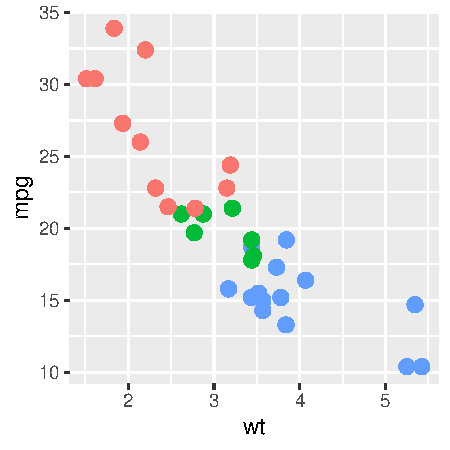
\includegraphics{Untitled3_files/figure-latex/figex-1} 

}

\caption{Narrow ggplot2 figure}\label{fig:figex}
\end{figure}

Here we use a standard knitr bloc with explicit options for

\begin{itemize}
\tightlist
\item
  figure width and height (\texttt{fig.width}, \texttt{fig.height}),
  both set to three inches;
\item
  whether the code is shown (\texttt{echo=TRUE}); and
\item
  the caption (\texttt{fig.cap}) as shown above.
\end{itemize}

\hypertarget{digital-figures}{%
\subsection{Digital Figures}\label{digital-figures}}

Markdown, Pandoc and LaTeX support \texttt{.eps} and \texttt{.pdf}
files.

Figures and Tables should be labelled and referenced in the standard way
using the \texttt{\textbackslash{}label\{\}} and
\texttt{\textbackslash{}ref\{\}} commands.

The R examples above show how to insert a column-wide figure. To insert
a figure wider than one column, please use the
\texttt{\textbackslash{}begin\{figure*\}...\textbackslash{}end\{figure*\}}
environment.

One (roundabout) way of doing this is to \emph{not} actually plot a
figure, but to save it in a file as the following segment shows:

\begin{Shaded}
\begin{Highlighting}[]
\KeywordTok{library}\NormalTok{(ggplot2)}
\end{Highlighting}
\end{Shaded}

\begin{ShadedResult}
\begin{verbatim}
#  Warning: package 'ggplot2' was built under R version 3.5.3
\end{verbatim}
\end{ShadedResult}

\begin{Shaded}
\begin{Highlighting}[]
\NormalTok{p <-}\StringTok{ }\KeywordTok{ggplot}\NormalTok{(}\DataTypeTok{data =}\NormalTok{ midwest,}
            \DataTypeTok{mapping =} \KeywordTok{aes}\NormalTok{(}\DataTypeTok{x =}\NormalTok{ area,}
                          \DataTypeTok{fill =}\NormalTok{ state,}
                          \DataTypeTok{color =}\NormalTok{ state)) }\OperatorTok{+}
\StringTok{    }\KeywordTok{geom_density}\NormalTok{(}\DataTypeTok{alpha =} \FloatTok{0.3}\NormalTok{)}
\CommentTok{## save to file}
\KeywordTok{suppressMessages}\NormalTok{(}\KeywordTok{ggsave}\NormalTok{(}\StringTok{"densities.pdf"}\NormalTok{, p))}
\end{Highlighting}
\end{Shaded}

This file is then included via standard LaTeX commands.

\begin{figure*}
  \begin{center}
    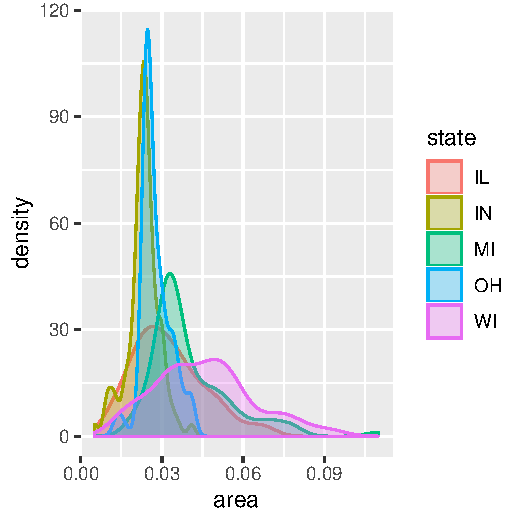
\includegraphics[width=0.66\textwidth, height=3.5in]{densities} 
  \end{center}
  \caption{Wide ggplot2 figure}\label{fig}
\end{figure*}

\hypertarget{typeset-code-but-do-not-run-it}{%
\subsection{Typeset Code (But Do Not Run
It)}\label{typeset-code-but-do-not-run-it}}

We can also just show code.

\begin{Shaded}
\begin{Highlighting}[]
\NormalTok{xx <-}\StringTok{ }\NormalTok{faithful[,}\StringTok{"eruptions"}\NormalTok{]}
\NormalTok{fit <-}\StringTok{ }\KeywordTok{density}\NormalTok{(xx)}
\KeywordTok{plot}\NormalTok{(fit)}
\end{Highlighting}
\end{Shaded}

This simply used a pandoc bloc started and ended by three backticks,
with \texttt{r} as the language choice. Similarly, \emph{many} other
languages can be typeset directly simply by relying on pandoc.

\hypertarget{single-column-equations}{%
\subsection{Single column equations}\label{single-column-equations}}

Authors may use 1- or 2-column equations in their article, according to
their preference.

To allow an equation to span both columns, options are to use the
\texttt{\textbackslash{}begin\{figure*\}...\textbackslash{}end\{figure*\}}
environment mentioned above for figures. The
\texttt{\textbackslash{}begin\{widetext\}...\textbackslash{}end\{widetext\}}
environment as shown in equation \ref{eqn:example} below is deprecated,
but \LaTeX commands \texttt{\textbackslash{}onecolumn} and
\texttt{\textbackslash{}twocolumn} work fine.

Please note that this option may run into problems with floats and
footnotes, as mentioned in the \href{http://texdoc.net/pkg/cuted}{cuted
package documentation}. In the case of problems with footnotes, it may
be possible to correct the situation using commands
\texttt{\textbackslash{}footnotemark} and
\texttt{\textbackslash{}footnotetext}.

\begin{equation}
  \begin{aligned}
(x+y)^3&=(x+y)(x+y)^2\\
       &=(x+y)(x^2+2xy+y^2) \\
       &=x^3+3x^2y+3xy^3+x^3. 
       \label{eqn:example} 
  \end{aligned}
\end{equation}

%\showmatmethods
\showacknow


\bibliography{curvature\_review.bib}
\bibliographystyle{jss}



\end{document}

